\documentclass{standalone}
\usepackage{tikz}
\usetikzlibrary{patterns, positioning}


\begin{document}
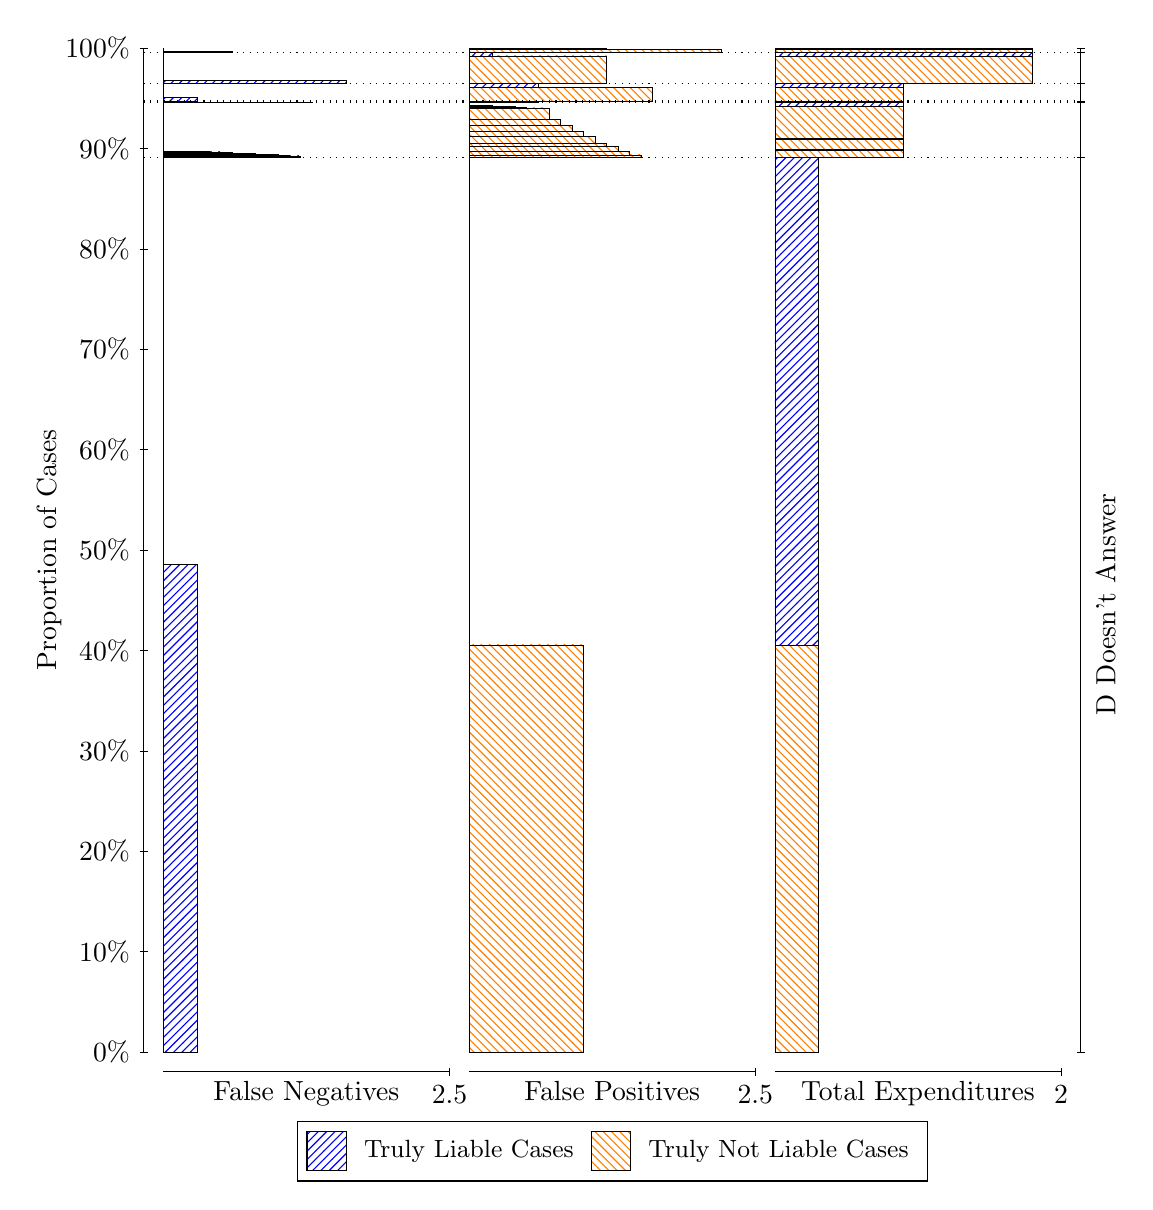
\begin{tikzpicture}
\draw[black, very thin] (1.5,1.75) -- (1.5,14.5);
\node[rotate=90, text=black, anchor=center] at (0.3, 8.125) {Proportion of Cases};
\draw[black, very thin] (1.45,1.75) -- (1.55,1.75);
\node[text=black, anchor=east] at (1.45, 1.75) {0\%};
\draw[black, very thin] (1.45,3.025) -- (1.55,3.025);
\node[text=black, anchor=east] at (1.45, 3.025) {10\%};
\draw[black, very thin] (1.45,4.3) -- (1.55,4.3);
\node[text=black, anchor=east] at (1.45, 4.3) {20\%};
\draw[black, very thin] (1.45,5.575) -- (1.55,5.575);
\node[text=black, anchor=east] at (1.45, 5.575) {30\%};
\draw[black, very thin] (1.45,6.85) -- (1.55,6.85);
\node[text=black, anchor=east] at (1.45, 6.85) {40\%};
\draw[black, very thin] (1.45,8.125) -- (1.55,8.125);
\node[text=black, anchor=east] at (1.45, 8.125) {50\%};
\draw[black, very thin] (1.45,9.4) -- (1.55,9.4);
\node[text=black, anchor=east] at (1.45, 9.4) {60\%};
\draw[black, very thin] (1.45,10.675) -- (1.55,10.675);
\node[text=black, anchor=east] at (1.45, 10.675) {70\%};
\draw[black, very thin] (1.45,11.95) -- (1.55,11.95);
\node[text=black, anchor=east] at (1.45, 11.95) {80\%};
\draw[black, very thin] (1.45,13.225) -- (1.55,13.225);
\node[text=black, anchor=east] at (1.45, 13.225) {90\%};
\draw[black, very thin] (1.45,14.5) -- (1.55,14.5);
\node[text=black, anchor=east] at (1.45, 14.5) {100\%};

\draw[black, very thin] (13.4,1.75) -- (13.4,14.5);
\draw[black, very thin] (13.35,1.75) -- (13.45,1.75);
\node[anchor=west] at (13.35, 1.75) {};
\draw[black, very thin] (13.35,13.115) -- (13.45,13.115);
\node[anchor=west] at (13.35, 13.115) {};
\draw[black, very thin] (13.35,13.812) -- (13.45,13.812);
\node[anchor=west] at (13.35, 13.812) {};
\draw[black, very thin] (13.35,13.827) -- (13.45,13.827);
\node[anchor=west] at (13.35, 13.827) {};
\draw[black, very thin] (13.35,14.048) -- (13.45,14.048);
\node[anchor=west] at (13.35, 14.048) {};
\draw[black, very thin] (13.35,14.44) -- (13.45,14.44);
\node[anchor=west] at (13.35, 14.44) {};
\draw[black, very thin] (13.35,14.5) -- (13.45,14.5);
\node[anchor=west] at (13.35, 14.5) {};

\draw[black, very thin, pattern color=blue, pattern=north east lines] (1.75,1.75) rectangle (2.186,7.9452);
\draw[black, very thin, pattern color=orange, pattern=north west lines] (1.75,7.9452) rectangle (1.75,13.115);
\draw[black, very thin, pattern color=blue, pattern=north east lines] (1.75,13.115) rectangle (3.494,13.131);
\draw[black, very thin, pattern color=blue, pattern=north east lines] (1.75,13.131) rectangle (3.3487,13.138);
\draw[black, very thin, pattern color=blue, pattern=north east lines] (1.75,13.138) rectangle (3.2033,13.146);
\draw[black, very thin, pattern color=blue, pattern=north east lines] (1.75,13.146) rectangle (3.058,13.15);
\draw[black, very thin, pattern color=blue, pattern=north east lines] (1.75,13.15) rectangle (3.058,13.152);
\draw[black, very thin, pattern color=blue, pattern=north east lines] (1.75,13.152) rectangle (2.9127,13.161);
\draw[black, very thin, pattern color=blue, pattern=north east lines] (1.75,13.161) rectangle (2.7673,13.166);
\draw[black, very thin, pattern color=blue, pattern=north east lines] (1.75,13.166) rectangle (2.622,13.174);
\draw[black, very thin, pattern color=blue, pattern=north east lines] (1.75,13.174) rectangle (2.4767,13.181);
\draw[black, very thin, pattern color=blue, pattern=north east lines] (1.75,13.181) rectangle (2.3313,13.188);
\draw[black, very thin, pattern color=orange, pattern=north west lines] (1.75,13.188) rectangle (1.75,13.812);
\draw[black, very thin, pattern color=blue, pattern=north east lines] (1.75,13.812) rectangle (3.6393,13.814);
\draw[black, very thin, pattern color=orange, pattern=north west lines] (1.75,13.814) rectangle (1.75,13.827);
\draw[black, very thin, pattern color=blue, pattern=north east lines] (1.75,13.827) rectangle (2.186,13.871);
\draw[black, very thin, pattern color=orange, pattern=north west lines] (1.75,13.871) rectangle (1.75,14.048);
\draw[black, very thin, pattern color=blue, pattern=north east lines] (1.75,14.048) rectangle (4.0753,14.089);
\draw[black, very thin, pattern color=orange, pattern=north west lines] (1.75,14.089) rectangle (1.75,14.44);
\draw[black, very thin, pattern color=blue, pattern=north east lines] (1.75,14.44) rectangle (2.622,14.461);
\draw[black, very thin, pattern color=orange, pattern=north west lines] (1.75,14.461) rectangle (1.75,14.5);
\draw[black, very thin, pattern color=orange, pattern=north west lines] (5.6333,1.75) rectangle (7.0867,6.9202);
\draw[black, very thin, pattern color=blue, pattern=north east lines] (5.6333,6.9202) rectangle (5.6333,13.115);
\draw[black, very thin, pattern color=orange, pattern=north west lines] (5.6333,13.115) rectangle (7.8133,13.142);
\draw[black, very thin, pattern color=orange, pattern=north west lines] (5.6333,13.142) rectangle (7.668,13.183);
\draw[black, very thin, pattern color=orange, pattern=north west lines] (5.6333,13.183) rectangle (7.5227,13.248);
\draw[black, very thin, pattern color=orange, pattern=north west lines] (5.6333,13.248) rectangle (7.3773,13.289);
\draw[black, very thin, pattern color=orange, pattern=north west lines] (5.6333,13.289) rectangle (7.232,13.377);
\draw[black, very thin, pattern color=orange, pattern=north west lines] (5.6333,13.377) rectangle (7.0867,13.441);
\draw[black, very thin, pattern color=orange, pattern=north west lines] (5.6333,13.441) rectangle (6.9413,13.515);
\draw[black, very thin, pattern color=orange, pattern=north west lines] (5.6333,13.515) rectangle (6.796,13.591);
\draw[black, very thin, pattern color=orange, pattern=north west lines] (5.6333,13.591) rectangle (6.6507,13.74);
\draw[black, very thin, pattern color=blue, pattern=north east lines] (5.6333,13.74) rectangle (6.36,13.747);
\draw[black, very thin, pattern color=blue, pattern=north east lines] (5.6333,13.747) rectangle (6.2147,13.754);
\draw[black, very thin, pattern color=blue, pattern=north east lines] (5.6333,13.754) rectangle (6.0693,13.762);
\draw[black, very thin, pattern color=blue, pattern=north east lines] (5.6333,13.762) rectangle (5.924,13.767);
\draw[black, very thin, pattern color=blue, pattern=north east lines] (5.6333,13.767) rectangle (5.7787,13.776);
\draw[black, very thin, pattern color=blue, pattern=north east lines] (5.6333,13.776) rectangle (5.6333,13.812);
\draw[black, very thin, pattern color=orange, pattern=north west lines] (5.6333,13.812) rectangle (6.5053,13.826);
\draw[black, very thin, pattern color=blue, pattern=north east lines] (5.6333,13.826) rectangle (5.6333,13.827);
\draw[black, very thin, pattern color=orange, pattern=north west lines] (5.6333,13.827) rectangle (7.9587,14.004);
\draw[black, very thin, pattern color=blue, pattern=north east lines] (5.6333,14.004) rectangle (6.5053,14.048);
\draw[black, very thin, pattern color=orange, pattern=north west lines] (5.6333,14.048) rectangle (7.3773,14.399);
\draw[black, very thin, pattern color=blue, pattern=north east lines] (5.6333,14.399) rectangle (5.924,14.44);
\draw[black, very thin, pattern color=orange, pattern=north west lines] (5.6333,14.44) rectangle (8.8307,14.479);
\draw[black, very thin, pattern color=blue, pattern=north east lines] (5.6333,14.479) rectangle (7.3773,14.5);
\draw[black, very thin, pattern color=orange, pattern=north west lines] (9.5167,1.75) rectangle (10.062,6.9202);
\draw[black, very thin, pattern color=blue, pattern=north east lines] (9.5167,6.9202) rectangle (10.062,13.115);
\draw[black, very thin, pattern color=orange, pattern=north west lines] (9.5167,13.115) rectangle (11.152,13.204);
\draw[black, very thin, pattern color=blue, pattern=north east lines] (9.5167,13.204) rectangle (11.152,13.213);
\draw[black, very thin, pattern color=orange, pattern=north west lines] (9.5167,13.213) rectangle (11.152,13.336);
\draw[black, very thin, pattern color=blue, pattern=north east lines] (9.5167,13.336) rectangle (11.152,13.348);
\draw[black, very thin, pattern color=orange, pattern=north west lines] (9.5167,13.348) rectangle (11.152,13.761);
\draw[black, very thin, pattern color=blue, pattern=north east lines] (9.5167,13.761) rectangle (11.152,13.812);
\draw[black, very thin, pattern color=orange, pattern=north west lines] (9.5167,13.812) rectangle (11.152,13.826);
\draw[black, very thin, pattern color=blue, pattern=north east lines] (9.5167,13.826) rectangle (11.152,13.827);
\draw[black, very thin, pattern color=orange, pattern=north west lines] (9.5167,13.827) rectangle (11.152,14.004);
\draw[black, very thin, pattern color=blue, pattern=north east lines] (9.5167,14.004) rectangle (11.152,14.048);
\draw[black, very thin, pattern color=orange, pattern=north west lines] (9.5167,14.048) rectangle (12.787,14.399);
\draw[black, very thin, pattern color=blue, pattern=north east lines] (9.5167,14.399) rectangle (12.787,14.44);
\draw[black, very thin, pattern color=orange, pattern=north west lines] (9.5167,14.44) rectangle (12.787,14.479);
\draw[black, very thin, pattern color=blue, pattern=north east lines] (9.5167,14.479) rectangle (12.787,14.5);
\draw[black, dotted] (1.5,13.115) -- (13.4,13.115);
\draw[black, dotted] (1.5,13.812) -- (13.4,13.812);
\draw[black, dotted] (1.5,13.827) -- (13.4,13.827);
\draw[black, dotted] (1.5,14.048) -- (13.4,14.048);
\draw[black, dotted] (1.5,14.44) -- (13.4,14.44);
\draw[black, very thin] (1.75,1.5) -- (5.3833,1.5);
\node[text=black, anchor=north] at (3.5667, 1.5) {False Negatives};
\draw[black, very thin] (5.3833,1.45) -- (5.3833,1.55);
\node[text=black, anchor=north] at (5.3833, 1.45) {2.5};

\draw[black, very thin] (5.6333,1.5) -- (9.2667,1.5);
\node[text=black, anchor=north] at (7.45, 1.5) {False Positives};
\draw[black, very thin] (9.2667,1.45) -- (9.2667,1.55);
\node[text=black, anchor=north] at (9.2667, 1.45) {2.5};

\draw[black, very thin] (9.5167,1.5) -- (13.15,1.5);
\node[text=black, anchor=north] at (11.333, 1.5) {Total Expenditures};
\draw[black, very thin] (13.15,1.45) -- (13.15,1.55);
\node[text=black, anchor=north] at (13.15, 1.45) {2};

\node[text=black, centered, rotate=90] at (13.72, 7.4327) {D Doesn't Answer};






\draw (7.449999999999999,1.5) node[draw=none] (baseCoordinate) {};
\begin{scope}[align=center]
        \matrix[scale=0.5, draw=black, below=0.5cm of baseCoordinate, nodes={draw}, column sep=0.1cm]{
            \node[rectangle, draw, minimum width=0.5cm, minimum height=0.5cm, pattern color=blue, pattern=north east lines] {}; &
            \node[draw=none, font=\small, text=black] (B) {Truly Liable Cases}; &
            \node[rectangle, draw, minimum width=0.5cm, minimum height=0.5cm, pattern color=orange, pattern=north west lines] {}; &
            \node[draw=none, font=\small, text=black] (B) {Truly Not Liable Cases}; \\
            };
\end{scope}

\end{tikzpicture}
\end{document}